\def\bra#1{\langle #1 \vert}
\def\ket#1{\vert #1 \rangle}
\def\braket#1#2{\langle #1 \vert #2 \rangle}
%\def\bind#1#2{\ket{#1}\bra{#2}}
\def\bind#1#2{\ket{#1}|\ket{#2}}
\def\bind#1#2{#1 \| #2}
\let\tilde\widetilde
\def\softmax#1{\mbox{Softmax}\left(#1\right)}
\def\emph#1{\vskip5pt\noindent{\it\bfseries #1}}
\def\task#1{\vskip5pt\noindent{\it\bfseries #1.}}
\def\qkv#1#2#3{\mbox{CrossAttention}(Q\!\leftarrow\!#1,\; K\!\leftarrow\!#2,\; V\!\leftarrow\!#3)}

\addtocounter{section}{2}
\section{Relational abstractors as transformer modules}

In the previous section relational learning 
in terms of symbolic message passing operations, where the connection to transformers 
was suggested. In this section, we make the connection more explicit, formulating 
these operations as extensions of transformer architectures.



\subsection{Relational learning using transformers}

In the abstractor framework, processing occurs in encoder/decoder modules that handle particular types of information, separated from modules for ``abstract inference.'' The encoders/decoders and the abstractor modules communicate through cross attention mechanisms that couple abstract states with specific information in encoder/decoder modules to which they refer in a given problem instance.  The abstract layers are composable to include a hierarchy of abstract modules in which higher order relations are learned from lower level relations, analogous to how convolutional layers are composed in deep neural networks.

The architecture has three types of states: encoder states $E$, decoder states $D$, and abstract states $A$. The encoder and decoder states are vectors
that represent domain-specific information (e.g., sensory or motor), which are often successfully modeled  
by standard deep learning frameworks, including standard transformers. The abstract states $A$ are vectors 
that are learned and processed using similar mechanisms but, critically, without direct exposure to the $E$ and $D$ states.  In particular, the encoder states are separated from the abstract states by a ``relational bottleneck'' 
that only allows information about relations (that is, inner-products) between encoder 
states to influence the transformation of abstract states.

\begin{figure}[t]
    \vspace{-3mm}
    \begin{center}
    \begin{tabular}{cc}
        \hskip2pt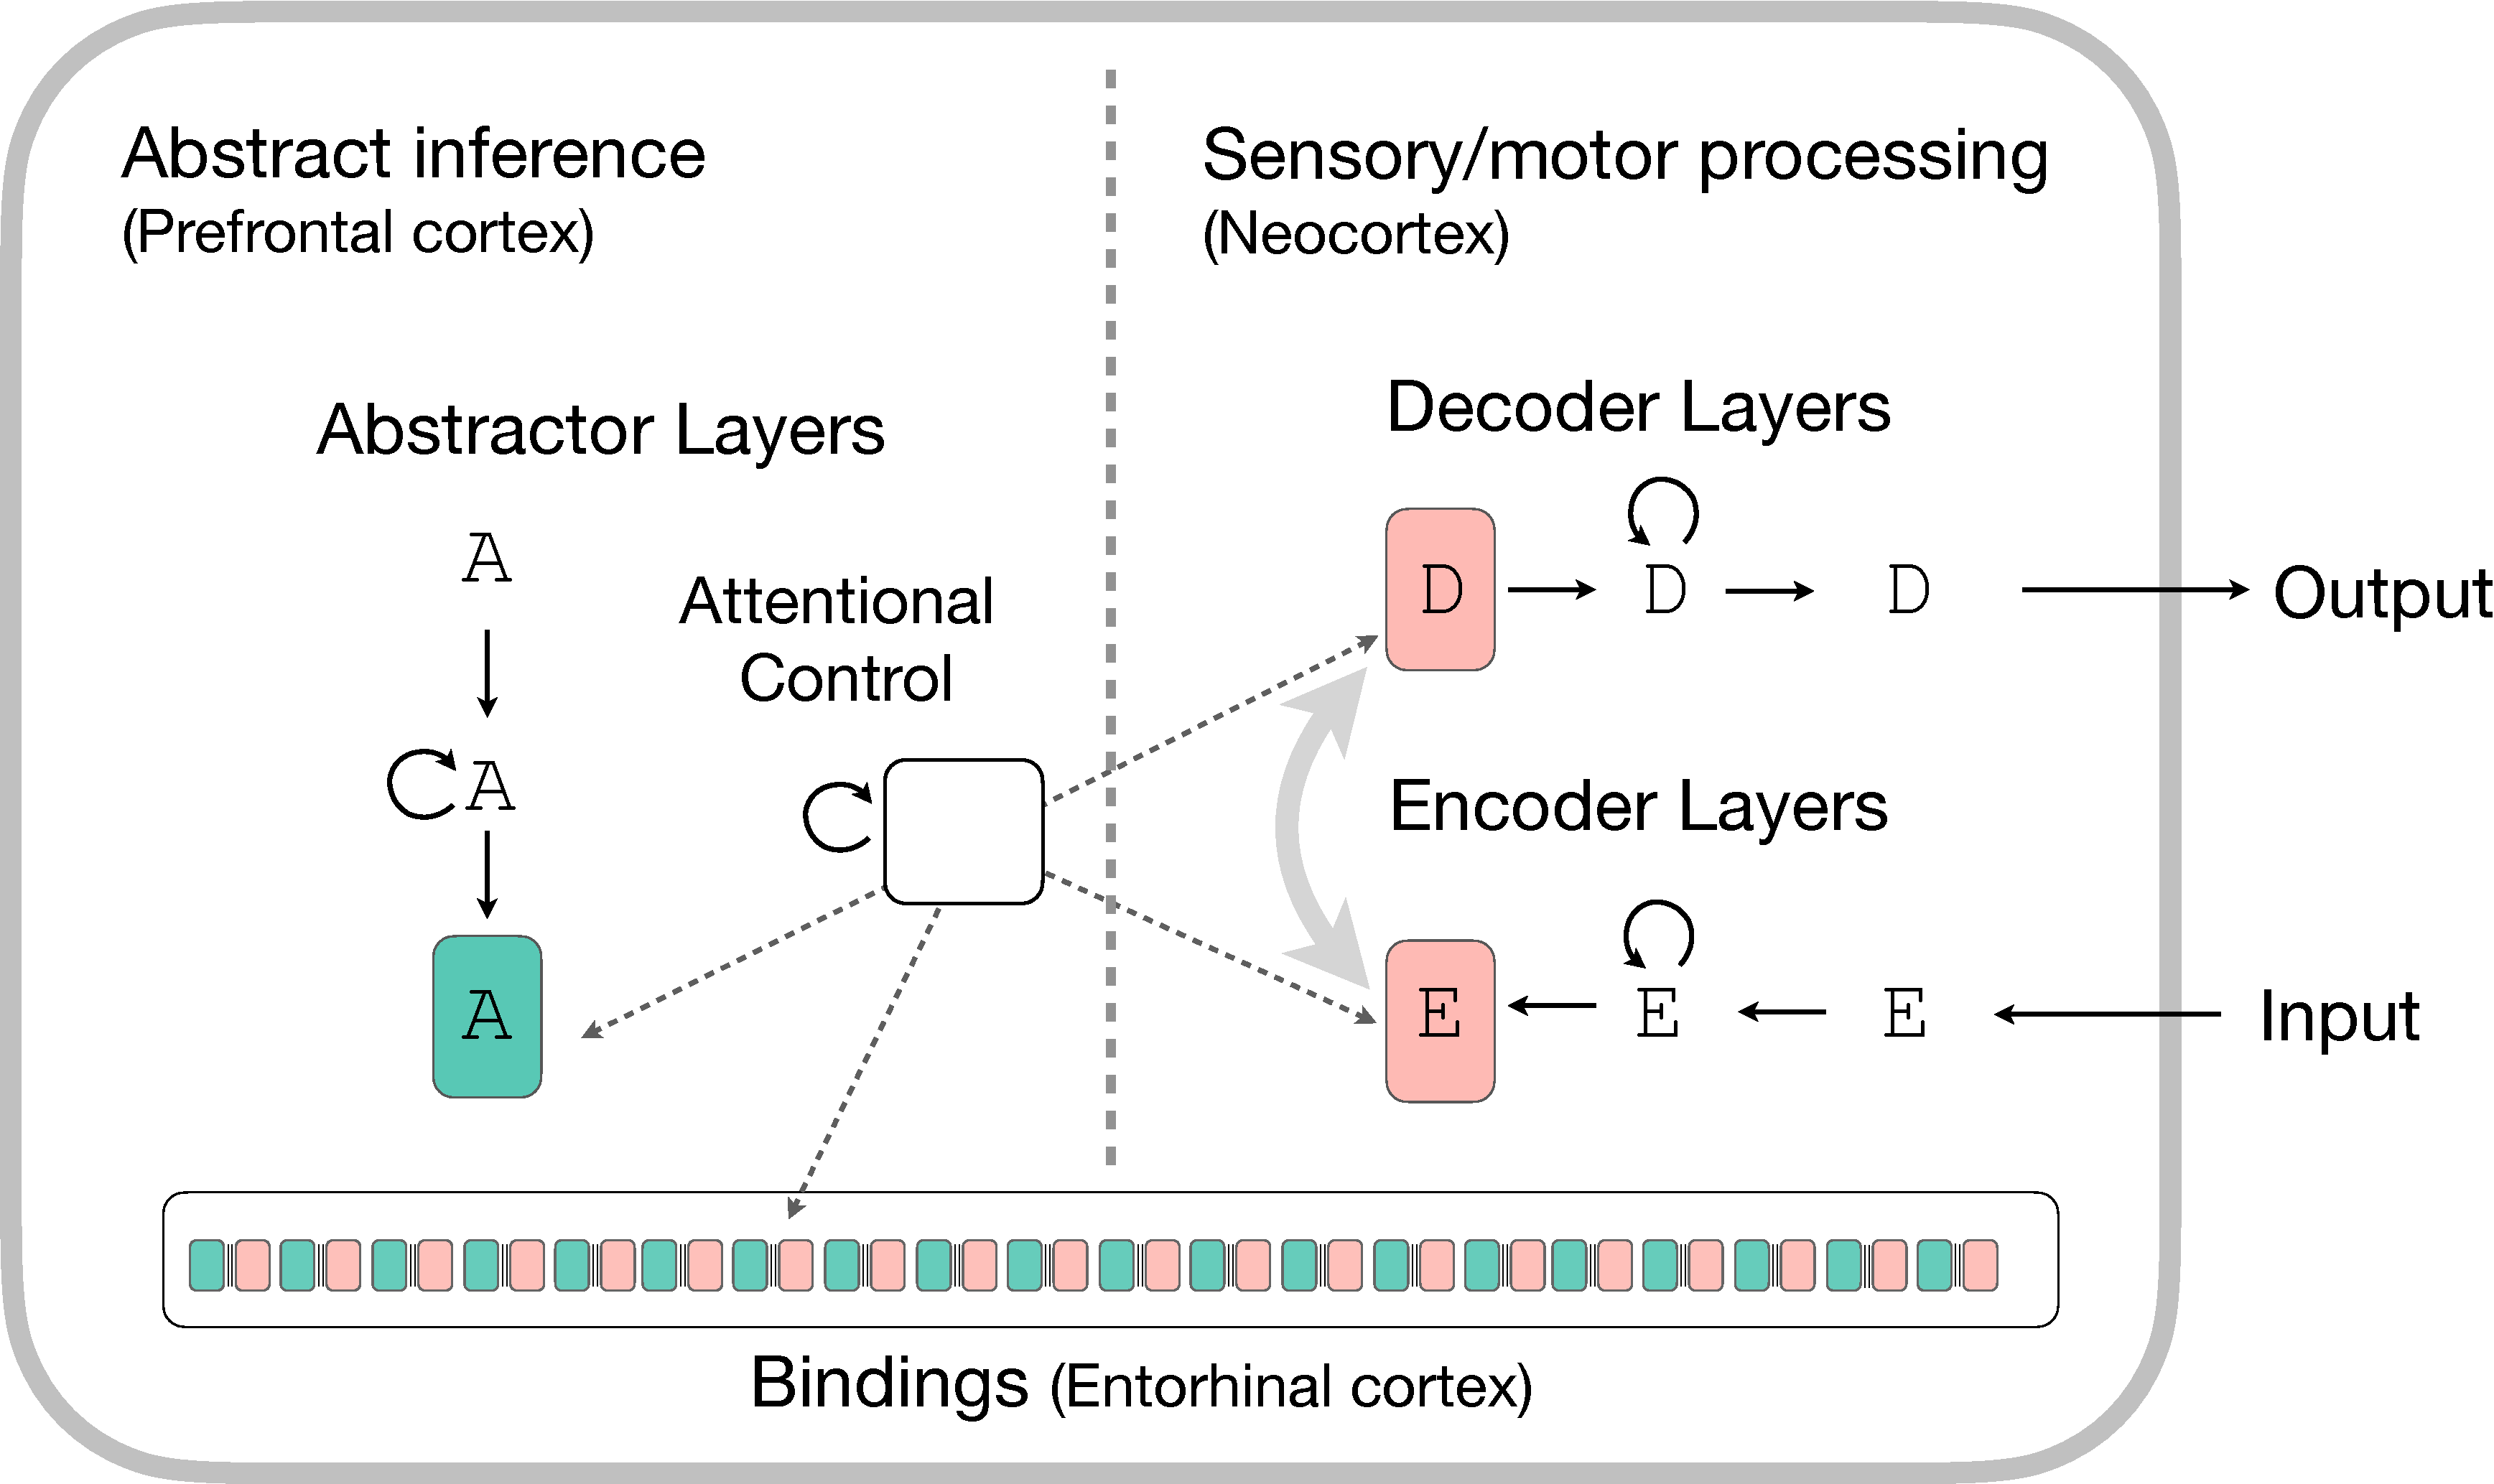
\includegraphics[width=.46\textwidth]{figures/algorithm-diagram2-crop} &
        \hskip5pt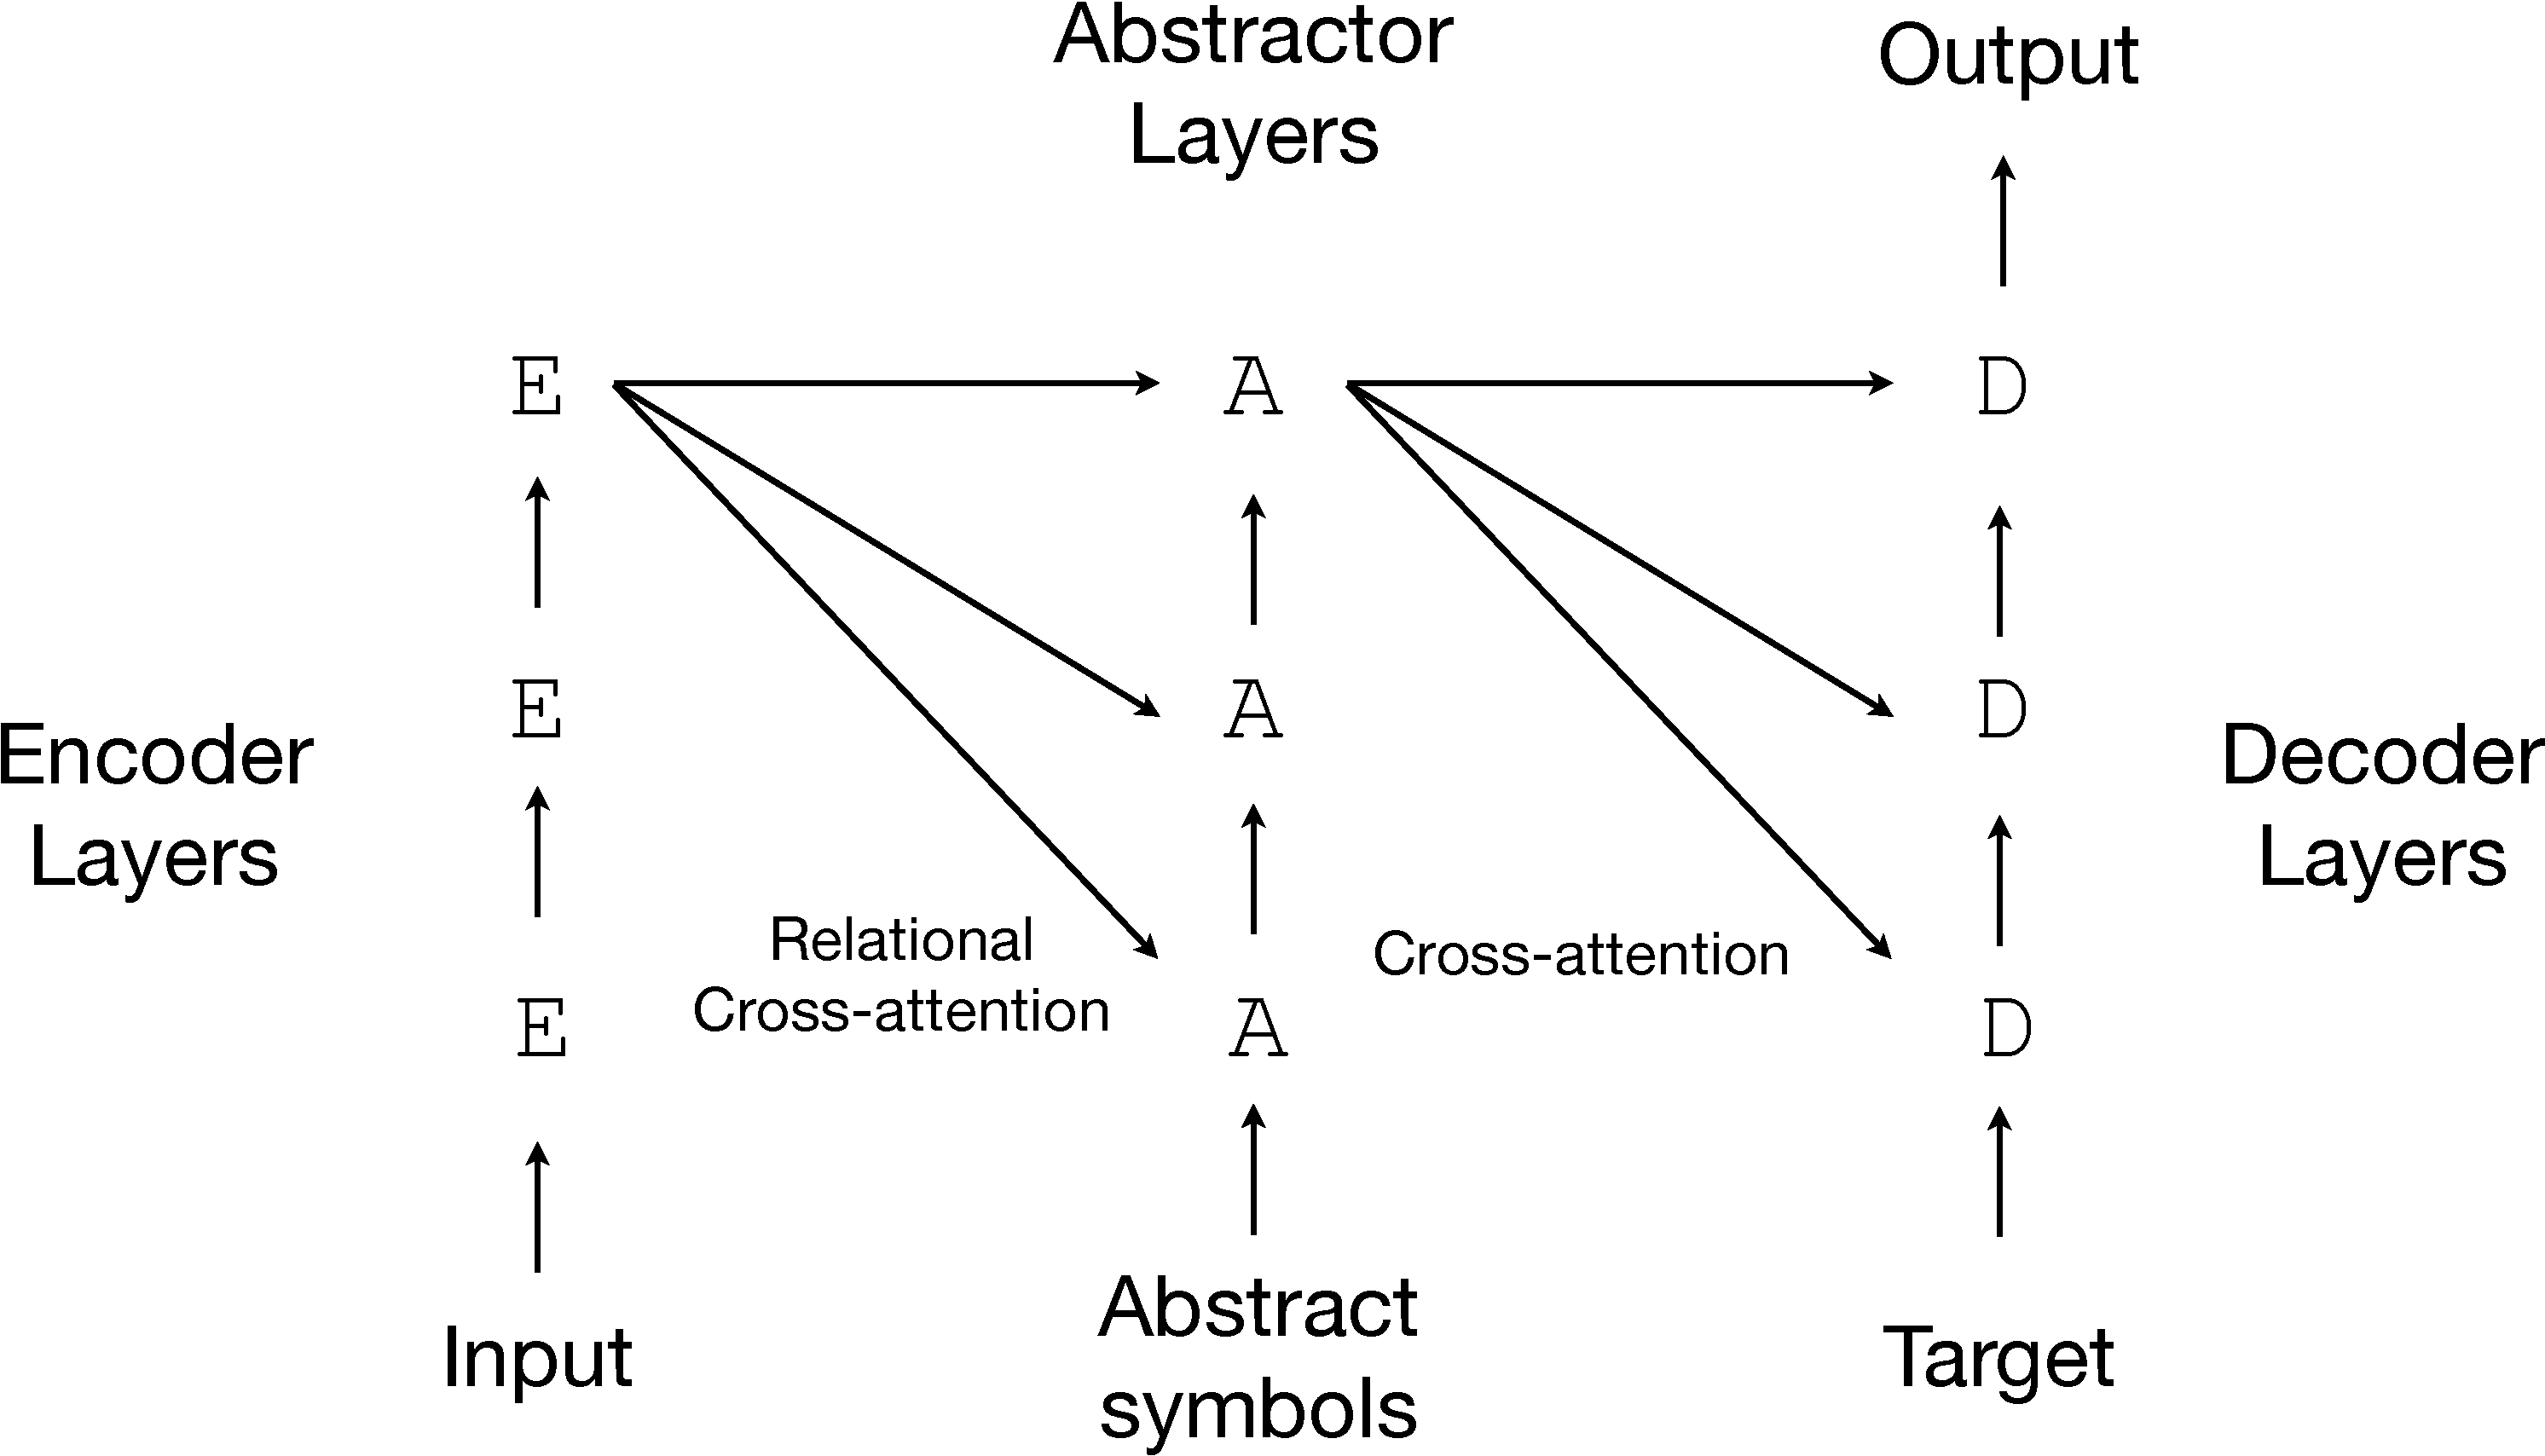
\includegraphics[width=.47\textwidth]{figures/algorithm-diagram3-crop} 
    \end{tabular}
    \caption{Algorithmic framework integrating transformers and relational learning, with encoder/decoder layers for sensory/motor processes, and abstractor layers for representing relations between encoder and decoder states. Left: In general, the relational cross attention mechanisms can be regulated by a controller, and bindings between encoder/decoder and abstractor states are maintained in episodic memory. The architecture is motivated by principles of brain organization separating sensory processing from abstract reasoning and decision making. Right: Simplification in terms of a transformer architecture, where the abstract symbols depend only on relations between encoder states. %This allows abstract states---e.g., emergent symbols---to be shared and reused across problems and %domains, leading to data efficiency and generalization. When Encoder/Decoder states appear together %repeatedly through experience and replay, the abstract inference circuit can be preempted by a direct %connection (gray arrow), leading to computational efficiency and parallelization (i.e., consolidation %and automatization). 
    }
    \label{fig:algo}
    \vskip-12pt
    \end{center}
\end{figure}

\subsection{Relational cross-attention}


In transformers, attention is used to access convex combinations of vectors called \text{values}. The weights are normalized inner products between other vectors called the keys and queries, after mapping each with a separate, learned linear transformation. If the queries are the columns of a matrix $Q = (q_1,\ldots, q_m)\in\reals^{d_1\times m}$, the keys are the columns of a matrix $K = (k_1, \ldots, k_m)\in\reals^{d_1\times m}$, and the values are the columns a matrix $V\in\reals^{d_2\times m}$, then the cross-attention mechanism computes the convex combination in the column space of $V = (v_1, \ldots, v_m)$ given by 
\begin{align*}
    & V R  \\
    & R \equiv \softmax{K^T Q}
\end{align*}
with  the $\softmax{\cdot}$ operation applied to the columns, so that the rows sum to one. The $m\times m$ matrix $R = (r_{ij})$ is thought of 
as a relation between keys and values, computed in terms of inner products, with column $r_j$ 
encoding the relations between query $q_j$ and the keys $k_1, k_2, \ldots, k_m$. Thus, the transformed 
values are 
\begin{equation*}
    v_j \leftarrow V r_j = \sum_{i=1}^m r_{ij} v_i .
\end{equation*}

In standard transformers, the cross-attention mechanism between encoder states $E$ and decoder states $D$
uses queries $Q = AD$, keys $K = BE$, and values $V = CE$, where the matrices $A,B,C \in\reals^{d\times d}$ are 
linear transformations learned for each attention head.  We denote this with the notation 
\begin{equation*}
     \qkv{D}{E}{E}
\end{equation*}
where the linear transformations $A, B, C$ are not shown. The self-attention for the encoder 
states is then
\begin{equation*}
    \qkv{E}{E}{E}
\end{equation*}

Given the context of the encoder states $E$, a sequence of abstractor layers transforms the abstract symbols $A = (a_1,\ldots, a_m)$, using two types of attention: Self-attention $\qkv{A}{A}{A}$ and 
\textit{relational cross-attention} 
\begin{equation*}
    \qkv{E}{E}{A}.
\end{equation*} 
The initial abstract state is $S = (s_1,\ldots, s_m)$ 
with abstract symbols $s_j$ that are task-dependent but input-indendent, trainable using 
backpropagation. The relational cross-attention mechanism learns relations among the encoder states and use those relations to transform the abstract state. Importantly, the relational cross-attention heads 
encode learned relations and attributes, and can be reused across tasks.


Only relational information in the encoder states, computed through inner products, 
is used to transform the abstract variables; no information about the encoder states $E$ is directly accessed by the abstract side. For example, an attention head may learn to be directed toward the relevant dimension of an $E$ state (e.g., the color or shape of an object), without being associated with any particular value along that dimension. If the specific representation of $E$ changes, the same abstract relations will hold as long as the transformed inner products are approximately preserved. 



\subsection{Example}

We use the game SET to illustrate relational cross-attention. SET is a relatively straightforward but challenging cognitive task that engages reasoning faculties in a deliberative, attentionally directed manner, requiring several levels of abstraction over sensory embeddings. Players are presented with 12 cards, each of which contains figures that vary along four dimensions (color, number, pattern, and shape; see Figure \ref{fig_set}a) and they must find subsets of three cards which obey a simple but challenging rule: along each dimension, all cards in a set must either have the same or unique values (e.g., in Figure \ref{fig_set}, cards with two solid blue/purple diamonds, two striped blue squiggles, and two open blue oblongs: same color, same number, different patterns, different shapes). 

Algorithmically, task performance can be described as follows. The visual arrangement of cards is processed into a set of encoder states $E$ by standard deep learning mechanisms. The abstractor, starting in some initial abstract state $A$, transforms the state by the evaluation of attention heads that extract relations between the cards, each head giving a relation between them in a learned attribute. 

\def\redcard{\colorbox{red!30}{R}\hskip.2em}
\def\bluecard{\colorbox{blue!30}{B}\hskip.2em}
\def\greencard{\colorbox{green!50}{G}\hskip.2em}
\def\onecard{\fbox{\hskip1pt 1\hskip1pt}\hskip.2em}
\def\twocard{\fbox{\hskip1pt 2\hskip1pt}\hskip.2em}
\def\threecard{\fbox{\hskip1pt 3\hskip1pt}\hskip.2em}

\begin{figure}[t]
\begin{center}
\begin{tabular}{ccc}
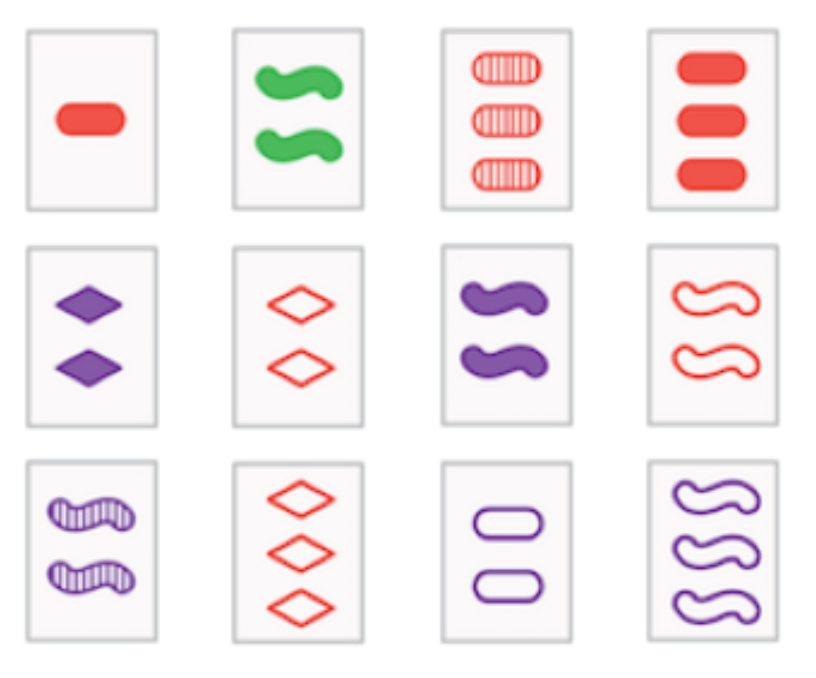
\includegraphics[width=.23\textwidth]{figures/set_example}
& &\\[-1.45in]
&\hskip10pt\ &\renewcommand{\arraystretch}{1.4}
\begin{small}
\begin{tabular}{|c|c|c|}
%\hline
\multicolumn{3}{c}{Attributes of encoder state $E=E_{1:3}$} \\
\hline
\multicolumn{1}{|c}{\redcard \redcard \redcard} & \multicolumn{1}{|c}{ \redcard\bluecard\greencard} &\multicolumn{1}{|c|}{\redcard\redcard\bluecard} \\
\hline
\hline
$\frac{1}{3}(A_1+A_2+A_3)$ & $\frac{1}{2}(A_2+A_3)$ & $A_3$ \\
$\frac{1}{3}(A_1+A_2+A_3)$ & $\frac{1}{2}(A_1+A_3)$ & $A_3$ \\
$\frac{1}{3}(A_1+A_2+A_3)$ & $\frac{1}{2}(A_1+A_2)$ & $\frac{1}{2}(A_1+A_2)$ \\
\hline
\multicolumn{3}{c}{Transformed abstract symbol $A=A_{1:3}$}
%\hline
\end{tabular}
\end{small}
%& \\[-1.45in]
%&&\includegraphics[width=.23\textwidth]{ppo-results/epoch_14_decision_boundaries} \vspace{-2mm} \\ 
\\[10pt]
\scriptsize (a) SET game && \scriptsize (b) Example of symbols/attention 
\end{tabular}
\vspace{-1mm}
\end{center}
\caption{Illustration of mechanism used in abstractor layers with relational cross attention using the game of SET (see text for description). 
%To provide a basic working of example of abstraction in our framework, 
As an example, consider an initial abstract symbol $A = A_{1:3}$ for three cards, and the color attribute.
%, for concreteness. 
Suppose a relation is learned such that  $\braket{E_i}{E_j}$ is large if cards $i$ and $j$ have different color, and is small if they are the same color.  Then relational cross-attention transforms the initial abstract symbol $A$ as shown in the above table. A multilayer perceptron can learn to discriminate between these three cases. Once learned, the symbol $A$ then can be used to represent abstract ``same/different'' relations for sequence of inputs.}
\label{fig_set}
\end{figure}


\begin{comment}
\def\redcard{\colorbox{red!30}{R}\hskip.1em}
\def\bluecard{\colorbox{blue!30}{B}\hskip.1em}
\def\greencard{\colorbox{green!50}{G}\hskip.1em}
\def\onecard{\fbox{\hskip2pt 1\hskip2pt}\hskip.1em}
\def\twocard{\fbox{\hskip2pt 2\hskip2pt}\hskip.1em}
\def\threecard{\fbox{\hskip2pt 3\hskip2pt}\hskip.1em}

\begin{figure}[htb]
\vspace{-2mm}
    \centering
    \begin{minipage}{0.46\linewidth}
        \centering
     %  \begin{table}[h]
\scriptsize
\centering
\begin{tabulary}{\columnwidth}{@{}p{0.1\columnwidth}p{0.25\columnwidth}p{0.25\columnwidth}p{0.2\columnwidth}@{}}
\toprule
Symbol  & \multicolumn{3}{c}{{Symbol mapped by relational cross attention $\braket{E}{E}\ket{A}$}}  \\
\cmidrule(r){1-1}     \cmidrule(lr){2-4}
%\toprule
$A_1$ & $(A_1+A_2+A_3)/3$ & $(A_2+A_3)/2$ & $A_3$ \\
\midrule
$A_2$ & $(A_1+A_2+A_3)/3$ & $(A_1+A_3)/2$ & $A_3$ \\
\midrule

$A_3$ & $(A_1+A_2+A_3)/3$ & $(A_1+A_2)/2$ & $(A_1+A_2)/2$ \\
 \bottomrule
Attributes $\bra{E}$: & \redcard \redcard \redcard & \redcard\bluecard\greencard & \redcard\redcard\bluecard \\
& \onecard \onecard \onecard & \onecard\twocard\threecard & \onecard\onecard\twocard
\end{tabulary}
%\end{table}
        \caption{Illustration of mechanism used in abstractor layers with relational cross attention using the game of SET (see text for description). 
%To provide a basic working of example of abstraction in our framework, 
As an example, consider an initial abstract symbol $A = A_{1:3}$ for three cards, and the color attribute.
%, for concreteness. 
Suppose a relation is learned such that  $\braket{E_i}{E_j}$ is large if cards $i$ and $j$ have different color, and is small if they are the same color.  Then relational cross-attention (approximately) transforms the initial abstract symbol $A$ as shown in the above table. A simple multilayer perceptron can learn to discriminate between these three cases with very little training data. Once learned, the symbol $A$ then can be used to represent abstract ``same/different'' relations for any triple of inputs, regardless of their sensory encoding.}
        \label{fig:perf-node}
    \end{minipage}%
        \hspace{3mm}%
  \begin{minipage}{.5\linewidth}
    \centering
    \includegraphics[width=\linewidth]{figures/pp_parallel.pdf}
    \caption {Parallelized execution of the \textit{Predator Prey XL} model.}
    \label{fig:perf-parallel}
 \end{minipage}%
\end{figure}
\end{comment}

\subsection{Configuring abstractors for different tasks}
\def\module#1{\mbox{\small\texttt{#1}}}

Abstractors can be used to approach a variety of relational learning tasks. In the case of classification 
or regression, the default architecture would be 
$$\module{Encoder} \rightarrow \module{Abstractor}$$
and the discriminant or regression function is computed as $f(A)$, where $A$ is the final abstract state.
For relational sequence-to-sequence tasks, the default architecture is 
$$\module{Encoder} \rightarrow \module{Abstractor} \rightarrow \module{Decoder}$$
In a ``fully relational'' task, the decoder can only attend to the abstractor, and therefore 
only uses relational information from the input. An example is sorting objects; we give 
experimental details for this example in Section~\ref{sec:experiments}.
In a ``partially-relational'' task, the decoder will attend to both the abstractor and encoder modules. In such cases, relational information is important to solving the task, but information about input ``values'' is 
also important. This provides an extension of general sequence-to-sequence models with transformers.


We note that learning higher order relations is made possible by composing 
abstractors, as in the architecture
$$\module{Encoder} \rightarrow \module{Abstractor} \rightarrow \module{Abstractor} \rightarrow \module{Decoder}.$$
Since a one-layer abstractor is able to compute arbitrary functions of each object's relations, 
chaining together abstractors allows the computation of relations on relations. We formalize 
these comments in Section~\ref{sec:function_spaces}.

